\documentclass[tikz,border=10pt]{standalone}
\usetikzlibrary{calc, intersections}

\begin{document}
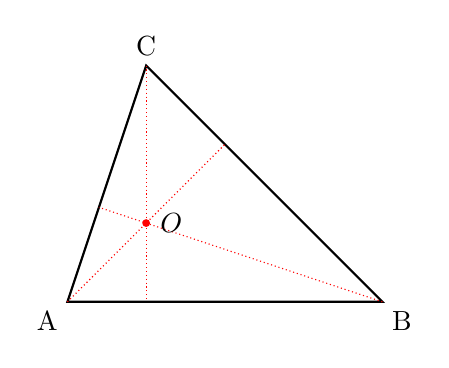
\begin{tikzpicture}
  % 三角形的垂心:Orthocenter
  % 定义顶点
  \coordinate[label=below left:A] (A) at (0,0);
  \coordinate[label=below right:B] (B) at (4,0);
  \coordinate[label=above:C] (C) at (1,3);
  
  % 绘制三角形
  \draw[thick] (A) -- (B) -- (C) -- cycle;
  
  % 计算垂足
  \coordinate (D) at ($(B)!(A)!(C)$); % A到BC的垂足
  \coordinate (E) at ($(A)!(B)!(C)$); % B到AC的垂足
  \coordinate (F) at ($(A)!(C)!(B)$); % C到AB的垂足
  
  % 绘制高线(红色虚线)
  \draw[red, densely dotted, name path=AD] (A) -- (D);
  \draw[red, densely dotted, name path=BE] (B) -- (E);
  \draw[red, densely dotted, name path=CF] (C) -- (F);
  \coordinate[name intersections={of=AD and BE, by=O}];
  \node[circle, inner sep=1pt, fill=red, label=right:$O$] at (O) {};   % 标记垂心
\end{tikzpicture}
\end{document}